% -----------------------------------------------
% Template for ISMIR Papers
% 2020 version, based on previous ISMIR templates

% Requirements :
% * 6+n page length maximum
% * 4MB maximum file size
% * Copyright note must appear in the bottom left corner of first page
% * Clearer statement about citing own work in anonymized submission
% (see conference website for additional details)
% -----------------------------------------------

\documentclass{article}
\usepackage[T1]{fontenc} % add special characters (e.g., umlaute)
\usepackage[utf8]{inputenc} % set utf-8 as default input encoding
\usepackage{ismir,amsmath,cite,url}
\usepackage{graphicx}
\usepackage{color}

% Optional: To use hyperref, uncomment the following.
\usepackage[bookmarks=false,hidelinks]{hyperref}
% Mind the bookmarks=false option; bookmarks are incompatible with ismir.sty.

\usepackage{lineno}
%\linenumbers
\newcommand{\carmine}[1]{\textbf{\color{red} Carmine => #1}}


% Title.
% ------
\title{Neural models for computer-assisted musical orchestration: a preliminary study}

% Note: Please do NOT use \thanks or a \footnote in any of the author markup

% Single address
% To use with only one author or several with the same address
% ---------------
%\oneauthor
% {Names should be omitted for double-blind reviewing}
% {Affiliations should be omitted for double-blind reviewing}

% Two addresses
% --------------
%\twoauthors
%  {First author} {School \\ Department}
%  {Second author} {Company \\ Address}

%% To make customize author list in Creative Common license, uncomment and customize the next line
%  \def\authorname{First Author, Second Author}


% Three addresses
% --------------
%\threeauthors
%  {First Author} {Affiliation1 \\ {\tt author1@ismir.edu}}
%  {Second Author} {\bf Retain these fake authors in\\\bf submission to preserve the formatting}
%  {Third Author} {Affiliation3 \\ {\tt author3@ismir.edu}}

%% To make customize author list in Creative Common license, uncomment and customize the next line
%  \def\authorname{First Author, Second Author, Third Author}

% Four or more addresses
% OR alternative format for large number of co-authors
% ------------
\multauthor
{First author$^1$ \hspace{1cm} Second author$^1$ \hspace{1cm} Third author$^2$} { \bfseries{Fourth author$^3$ \hspace{1cm} Fifth author$^2$}\\
  $^1$ Department of Computer Science, University , Country\\
$^2$ International Laboratories, City, Country\\
$^3$  Company, Address\\
{\tt\small CorrespondenceAuthor@ismir.edu, PossibleOtherAuthor@ismir.edu}
}
\def\authorname{First author, Second author, Third author, Fourth author, Fifth author}


\sloppy % please retain sloppy command for improved formatting

\begin{document}

%
\maketitle
%
\begin{abstract}
In this paper we will explore preliminary neural models for the task of computer-assisted musical orchestration. After an introduction on the problem, we will show how we decided to model musical orchestration as a classification task. In this context, we will propose two deep learning models and we will show how they perform as classifiers for musical instruments recognition by comparing them with specific baselines. We will the show how they perform, both qualitative and quantitative, in the task of computer-assisted orchestration by comparing them with state-of-the-art systems. We will highlight, finally, benefits and problems of neural approaches for orchestration and we will propose possible future steps.
\end{abstract}
%
\section{Introduction}\label{sec:introduction}

Computer-assisted orchestration is an important problem ... \carmine{Can you add more?}.

The approach studied in \cite{Cella19} consists in finding a good orchestration for any given sound by successive iterations, exploring a feature space defined by a fixed feature function $f$. This method is currently considered state of the art and was implemented in Orch-Idea.\\

In this paper, we try a different approach, using Deep Neural networks. The main idea is to train a model to classify combinations of real instruments, and use it then for orchestration. By training it with real combinations of instruments, such as \{Flute C6, Bassoon C4, Bassoon G4\}, the model will hopefully acquire the ability to identify the presence of each instrument and its associaed pitch by building the appropriate filter. Thus, when a sound is given as input, those filters will identify what are the best instruments that match the target sound.\\

This method is motivated by the good results obtained in previous research on musical instruments identification \cite{Benetos07}\cite{Kitahara05}\cite{Chetry05} and the more recent use of deep neural networks for musical classification \cite{lostanlen16}\cite{Bian}\cite{Brunner}\cite{Defossez19}. \carmine{Can you check if those references are good to use in this context?}\\

\iffalse
We attempt to use neural networks to solve the assisted orchestration problem. Our model must be able to take in a sound and identify what instruments playing which notes best represents the sound. Our idea is to frame this as a classification problem, where each class is an instrument-note pair. Our classifiers will be trained on sounds that are combinations of multiple instruments and notes, leading to a model that can take a complex mixture of timbres and deconstruct it into individual instrument-note pairs. When a new sound, one that is not simply a mixture of notes, is fed to the model, the predictions are used to create an orchestrated solution.

\fi

The features we use are the mel spectrogram of the input sound, because of its ability to represent the way we hear sounds and its common use in MIR\textbf{Reference}.\\

We found that even on a simplified version of this classification problem, parametric classifiers were unable to meaningfully identify instrument-note pairs as the number of instruments used in the combinations increased. Therefore the need for neural networks arose. The two architectures we used are a Convolutional Neural Network (CNN) with a Long Short-Term Memory (LSTM) unit, and ResNet, a well known residual architecture that already yielded good results for image classification \cite{He15}. We chose to use a CNN because of its success in audio classification \cite{Hershey16}. Our inclusion of an LSTM is because of its ability to learn long term dependencies in data \cite{Hochreiter97}, which is important given the temporal nature of audio.\\

After training these models on varying combinations of 10 instruments, we used them for orchestration. More specifically, we orchestrated 15 target sounds by feeding them to the networks and synthesizing a solution from the most likely samples output from the system. We then compared our orchestrations to OrchIdea's solutions for the same targets through both qualitative and quantitative means. For quantitative comparison, we computed a distance metric on the FFTs of the target and solution, comparing the distance between OrchIdea's solution and the target and our model's solution and the target. \carmine{Do we need to reference the use of that distance?}

Our codebase can be found at: \url{https://github.com/dzluke/DeepOrchestration}.
\section{Data}

\subsection{Data Source and Generation}

We used the TinySOL database to create our input data. TinySOL is a subset of the Studio On Line (SOL) database created by IRCAM \textbf{Reference needed}. TinySOL contains 1,529 samples from 12 instruments. The instruments come from different orchestral families: strings, woodwinds, and brass. Each sample is one instrument playing a single note in the ordinario style, with one of three dynamics: \textit{pp}, \textit{mf}, or \textit{ff}. The instruments and ranges over which they were recorded is summarized in Tab.\ref{tinysol}.  \carmine{Can you review this part about TinySOL and add more details if needed?}\\


We generated all the data we used to train our models based on the samples of TinySOL. For a given $N$, each input to our model is a combination of $N$ TinySOL samples chosen among an orchestra of 10 instruments. The data is generated in the following way: 

\begin{itemize}
\item We iteratively choose a random instrument, pitch and dynamic to pick the sample. We repeat that step $N$ times. Note that we don't allow the same instrument to be chosen more than three times in order to ensure variety in the mixtures.
\item The chosen samples are additively combined to be played simultaneously and normalized by the number of instruments.
\item The mel spectrogram of the mixture is computed to be used as the features input to the model.
\end{itemize}

The choice of using the mel spectrogram as input features of the model is very commmon in music information \cite{Stevens37} and can be considered to be an accurate representation of the way humans perceive sound and music.\carmine{Do we need more references for mel spectrogram?}\\

Samples had a sample rate of $44100$Hz and were all padded or chopped to be exactly 4 seconds long. The Mel spectrograms were then generated using an FFT hop length of 2048 samples (e.g. the window of each FFT was $46$ms wide), and a number of Mel bins equal to 128. Therefore, all the features fed to the model were matrices of size $128\times 345$. We used Librosa package in Python to compute the features, and more details on the exact computations can be found in \cite{mcfee15} The choice of the hop length was made by doing a compromise between the amount of information extracted by each FFT window, and the ability to capture changes in the dynamic, assuming that no change faster than $10$ms could be perceived by the human ear \carmine{Do you have a reference for that? I don't find anything on the topic}.

\begin{table}
\begin{tabular}{|c|c|c|}
\hline
Instrument & Abbreviation & Range \\
\hline
Violin & Vn & G3-E7\\
Cello & Vc & C2-C6\\
Viola & Va & C3-C7\\
Trumpet C & TpC & F\#3-C6\\
Trombone & Tbn & A\#0;A\#1-C5\\
Oboe & Ob & A\#3-A6\\
Horn & Hn & G1-F5\\
Flute & Fl & B3-D7\\
Clarinet Bb & ClBb & D3-G6\\
Contrabass & Cb & E1-C5\\
Bass Tuba & BTb & F\#1-F4\\
Bassoon & Bn & A\#1-D\#5\\
\hline
\end{tabular}
\caption{Table showing the pitch ranges present in the TinySOL database.\label{tinysol}}
\end{table}

\subsection{Data Augmentation}

In order to increase variability in our generated data, we used two methods of data augmentation \cite{Salamon17}\cite{Bhardwaj17} : pitch shifting and partial feature dropout.\\

The first one was done on the TinySOL samples. We performed a slight pitch shift by shifting the frequency of the signal. We did this by reading the samples with different sample rates. Python package librosa automatically converts the data coming from the samples to match the specified sample rate \cite{mcfee15}. Thus, a small difference in sample rate will slightly modify the perceived pitch if played at the normal sample rate. In practice, the sample rates used for this data augmentation were within $5\%$ of the actual $44100$Hz.\\

The second augmentation was performed on the feature matrix itself, the mel spectrogram. We chose random columns and rows of the matrix to zero out. For a given matrix, each column and each row had individually a $1\%$ chance to be set to 0, which yielded an average of $1.28$  columns and $3.45$ rows being zero-ed out. This method of data augmentation aimed to be more resilient to the possible errors of recording \carmine{Is there any other reference to justify this sentence?}, due either to a setup that induces interferences and cancels specific frequencies, or to a default in the microphone that fails to record a small temporal portion.

\section{Our model}

Our idea is to perform orchestration using deep neural networks trained for classification. In our setting, each class is an instrument-note pair. Our model takes in the mel spectrogram of a soundfile that is a combination of different instruments and pitches, and attempts to identify which instrument-pitch pairs are present. The network learns how to take a sound that is a complex combination of notes and timbres and deconstruct it into its original parts. Then, when a network is given a target sound as input, it will attempt to apply the same classification rules, outputting a vector of the probabilities of each sample being in the target sound. By taking the samples that have the highest probability, an orchestrated solution can be created. Both of our deep models use the Adam optimizer, Binary Cross-Entropy loss, and were written using PyTorch.

\subsection{Baseline}
In order to have a baseline to compare our results against, we attempted to solve the classification problem using various parametric classifiers. The classifiers we tested were Support Vector Machine (SVM), Random Forest, and K-Nearest Neighbors. We used the implementations provided in the scikit-learn library for Python \cite{scikit-learn}. For SVM, we used SVC with a non-linear RBF kernel. For Random Forest, we set the maximum depth of each tree to be 15.  All of the following baseline experiments used 50,000 generated samples with a train-test split of 60/40. Each sample is a combination of one or more instruments and is four seconds in length. The features used are the mel frequency cepstral coefficients (MFCCs) of the resulting combination, with a total of 100 coefficients per sample. We chose to use MFCCs for this setting because using the mel spectrogram leads to a number of features that is too high for the parametric classifiers. We found SVM to have the highest accuracy of the three classifiers across all experiments.

We found that the parametric classifiers were not able to solve the full setting of our problem which had 424 classes, so we started by simplifying the problem to classifying only the instruments and not the pitch. This had the benefit of both reducing the number of classes and increasing the number of samples per class. We found that SVM was able to very accurately identify the instrument given an input that had only one instrument present; for this case the accuracy was 99.8\%. However as soon as multiple instruments were present in the input, the accuracy dropped significantly. With two instruments, accuracy was 55.4\%, with three it was 19.6\% and with 10 instruments the accuracy was 0.5\%. K-Nearest Neighbors performed significantly worse than SVM, so we did not attempt any further testing with KNN.

To better approximate the problem of identifying instrument and pitch, we performed experiments in which two instruments were selected and for input data that contained samples from one of those two instruments, both the instrument and pitch class of the sample would be classified. That is, which octave the pitch was in did not matter, only the pitch class. The input was a combination of two instruments drawn from a possible twelve instruments, and the classifier attempted to identify which instruments were present and for the specified instruments, say Violin and Viola, which pitch classes were present. If another instrument was present in the input combination that was not Violin or Viola, the classifier would simply identify that an instrument that was not one of the two was present. The accuracies from this experiment are outlined in Table 1. Since Random Forest performed worse than SVM is every experiment, we stopped testing with Random Forest and used SVM from that point on.

We then performed this same experiment with three instruments having their pitch class identified. Flute, Oboe, and Violin reached an accuracy of 11.1\%, and Bass Tuba, Trumpet, and Trombone was 0.5\%. As we increased the number of instruments whose pitch classes was being identified, the accuracy continued to drop. For classifying the pitch class of four instruments: Oboe, French Horn, Violin, and Flute, the accuracy was 2.7\%.

This was still a simplified version of the problem, as we were identifying only the pitch class of a few instruments. However, the parametric classifiers were unable to achieve accurate results as the number of instruments increased. Therefore, we did not attempt the full setting of the problem, in which individual pitches are classified for all instruments, with parametric classifiers. 

\begin{table}
  \begin{center}
    \label{tab:table1}
    \begin{tabular}{|c|c|c|c|} 
    	  \hline
      \textbf{Instr. 1} & \textbf{Instr. 2} & \textbf{SVM Acc.} & \textbf{RF Acc.}\\
      \hline
      Violin & Flute & 38.8\% & 9.8\% \\
      \hline
      Violin & Trumpet & 33.8\% & 9.1\% \\
      \hline
      Violin & Cello & 34.8\% & 6.3\% \\
      \hline
      Cello & Viola & 32.1\% & 5.8\% \\
      \hline
      Oboe & French Horn & \textbf{39.9\%} & \textbf{17.5\%} \\
      \hline
    \end{tabular}
  \end{center}
  \caption{Comparison of accuracies between SVM and Random Forest. Each data point is a combination of two TinySOL samples, where at least one of the samples is from one of the two instruments specified for that experiment. For the samples drawn from one of the two instruments, the pitch class of that sample is identified. For a sample not from one of the two instruments, the classifier simply attempted to identify that a sample from one of the non-specified instruments was present. In this setting, there are 25 classes: 24 from the 12 pitch classes from 2 instruments, and 1 class that specified whether an instrument that is not one of the two specified is present.}
\end{table}


\subsection{CNN with LSTM}

The first deep model we tested was a Convolutional Neural Network (CNN) with a Long Short-Term Memory (LSTM) unit. CNNs show good performance on classification problems for their ability to extract spatial features, and have shown success in audio classification \cite{Hershey16}. Long Short-Term Memory (LSTM) units provide a way to learn long term dependencies in the data \cite{Hochreiter97}, which is relevant given the sequential nature of audio.

\carmine{Do we need any more justification on why we used that model?}

Our architecture contains four convolutional layers and two fully connected layers. Each convolutional layer is followed by a BatchNorm layer, a ReLU activation layer and a $2 \times 2$  MaxPool layer with a stride of 2. The kernel size is $3 \times 3$ with a stride of 1 and a padding of 1. The number of filters are 8, 16, 32, and 32.

Following the first three convolutional layers, there is an LSTM layer with 32 outputs. After the LSTM layer, there is a final convolutional layer yielding a tensor of dimensions $32\times 8 \times 21$. We flatten the outputs and feed them into fully a connected layer with Dropout, then another another fully connected layer. Finally, the sigmoid function is applied to the final layer. 

\carmine{Does this architecture need to be explained in more details?}

Since each class is independent, we are able to take the sigmoid activation and use binary classification for each class. The model architecture is shown in Figure \ref{cnn_lstm}.

\begin{figure*}
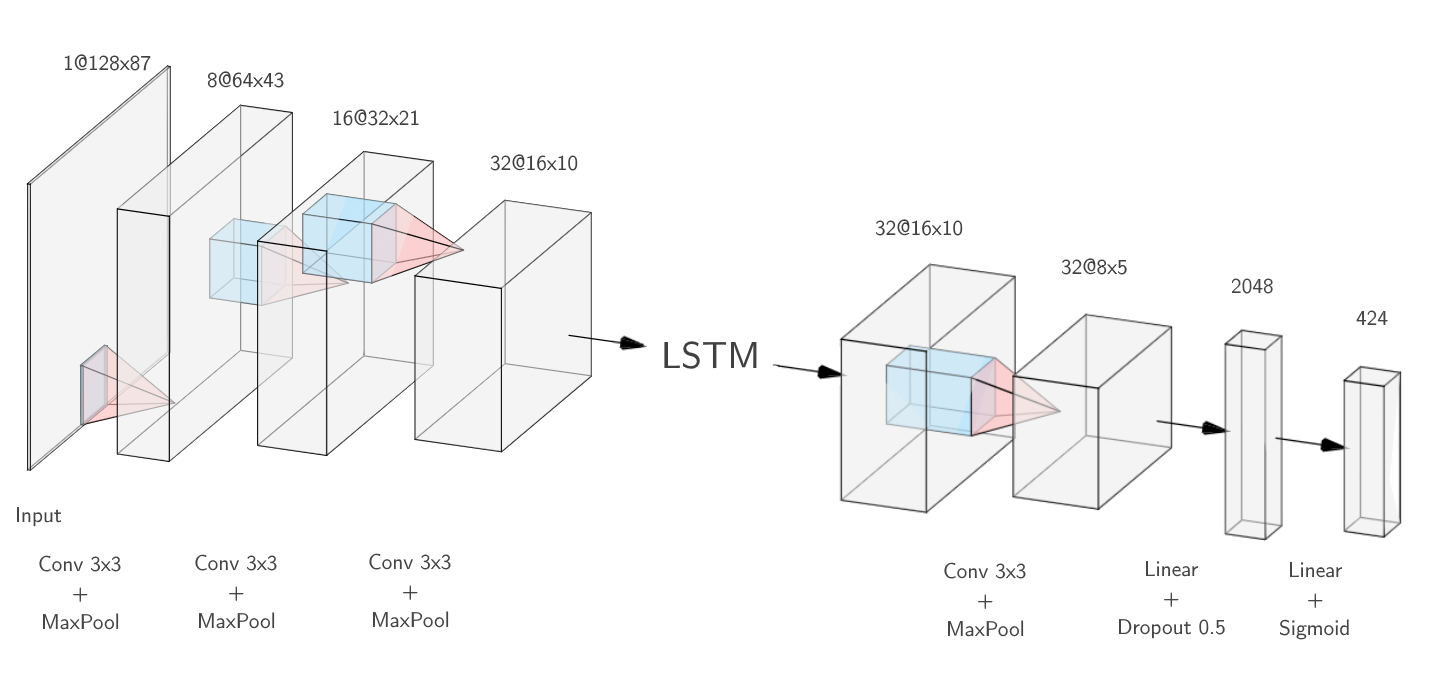
\includegraphics[scale=0.45]{CNN_LSTM_diagram.png}
\caption{Diagram of the CNN with LSTM architecture. \label{cnn_lstm}}
\end{figure*}


\subsection{ResNet}
\carmine{Can you add more to this section about why ResNet is good, and maybe some details about the implementation?}
The second deep model that we used was the well known deep residual network ResNet.

To make our setting more reasonable, we took the well-known deep residual network (ResNet) as backbone in our experiments. Specifically, we used 18-layer ResNet, which allows information to pass directly from the input to the final layer of each block. Besides, to make the model more suitable to our problem, we reduce the number of parameters and reset the output channel numbers of each block with 32, 64, 32, 32 respectively.

\subsection{Classification results}

During training, the loss function used to optimize the inner parameters of the model was binary cross entropy, as it is the common choice for multiclass multilabel classification frameworks such as this one \carmine{Is there a specific paper justifying that claim? Or is it obvious enough?}. However, the value of the loss function alone is difficult to interpret. For this reason we created a complementary function $f$ to be used only for evaluation. This function compares a vector of expected outputs $\overline{X}$ with the estimated output from the model $\hat{X}$ by using the following function

\begin{equation}
f(\overline{X}, \hat{X}) = \frac{1}{N}<\overline{X}, M_N(\hat{X})>
\label{eval}
\end{equation}

where

\begin{equation}
M_N(\hat{X})_i = \left\{\begin{array}{ll}
1 \text{ if } i \in I_N(\hat{X})\\
0 \text{ otherwise}
\end{array}\right.
\label{NMax}
\end{equation}
and $I_N(\hat{X})$ is the set of indices containing the $N$ first maximums of the vector $\hat{X}$.

More specifically, the function $M_N(\hat{X})$ takes as an input a vector of probabilities and outputs a vector where only the positions of the $N$ first maxima are set to 1. This new vector would be the orchestration of $N$ instruments given by the model. Thus, the function $f$ simply outputs the proportion of the estimated orchestration that matches the expected one.

Different experiments were made by varying the number $N$ of samples in each mixture sample. We used an orchestra of 10 instruments containing Horn, Oboe, Violin, Viola, Cello, Flute, Trombone, Bassoon, Trumpet C and Clarinet Bb.

Then, for both CNN with LSTM and ResNet, we computed the maximum accuracy over the epochs. For the CNN model, all the trainings with different values of $N$ were made using a dataset containing 200000 samples over 50 epochs, whereas for the ResNet, the dataset contained 400000 samples and was trained over 20 epochs. Fig. \ref{cnn_vs_resnet} shows the best overall test accuracy achieved by both models across the number of samples $N$.\\


\begin{figure}
\center{
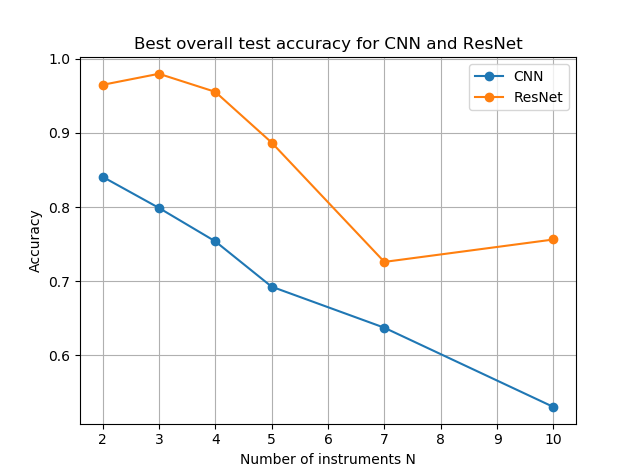
\includegraphics[scale=0.4]{figs/CNN_vs_ResNet.png}}
\caption{Best overall accuracy for CNN with LSTM and ResNet depending on the number of instruments in the combinations used for training. \label{cnn_vs_resnet}}
\end{figure}

From this plot, we see that ResNet achieves better performances than the CNN regardless of the number of samples used in the combination. This result isn't surprising as residual networks usually perform better for this kind of classification problems \carmine{It would need a citation on why ResNet was expected to be better}

Fig. \ref{best_acc_cnn} and Fig. \ref{best_acc_resnet} show the maximum accuracy computed using the function $f$ explicited in (\ref{eval}). Note that for ResNet, the variance of accuracy is much smaller until $N$ reaches 5 before becoming similar to the CNN. The results on both figures show consistency on the relative accuracy of instruments, which is a first step towards the validation of this method \carmine{Can I say that?}. Flute, Trombone and Trumpet yield the worst results for both models, being notably worst, which could be explained by the nature of their spectra. For the Flute, since it has very few harmonics, it is difficult to identify it among other instruments, especially if they are richer. On the other hand, brasses have a very rich spectra and a strong noisy component that excites almost all the frequencies.\\
Strings give consistent results, having for both models similar accuracies, an interesting point to notice is the very high accuracy of Oboe on both models. This could indicate that there is an optimal balance of harmonies that maximizes the probability of being detected in such classification framework.\carmine{Please review those interpretations}


\begin{figure}
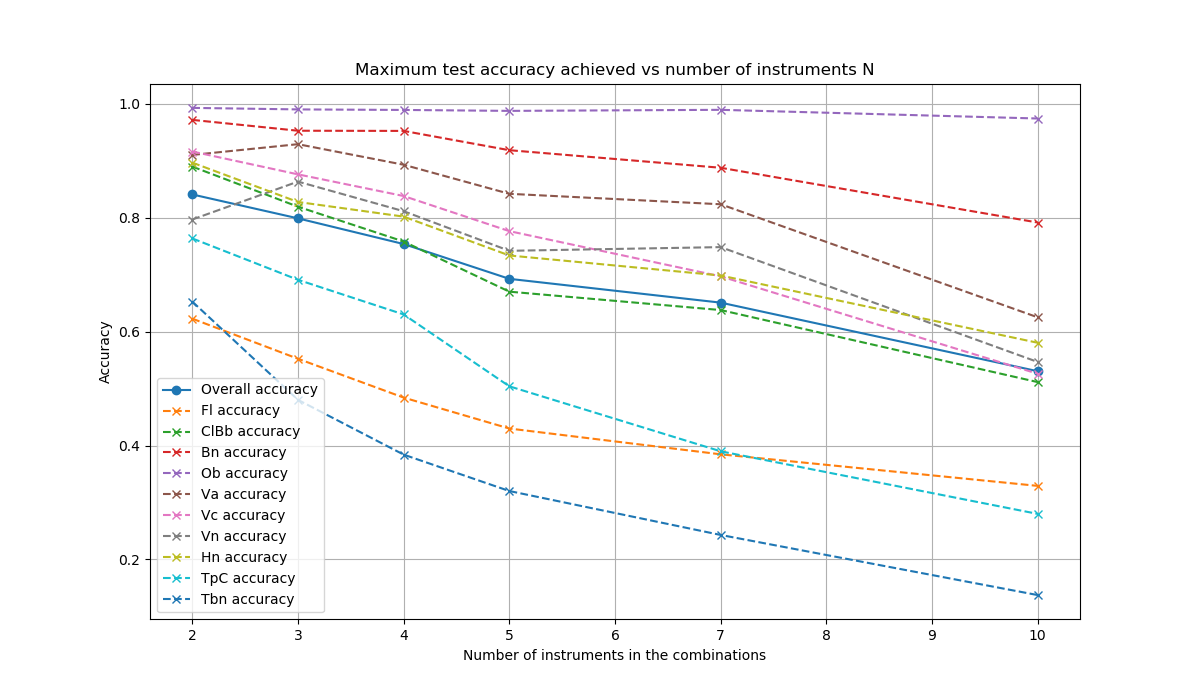
\includegraphics[scale=0.5]{figs/Acc_vs_N_CNN.png}
\caption{Best overall accuracy and for each instrument obtained by the CNN with LSTM depending on the number of instruments in the combinations. \label{best_acc_cnn}}
\end{figure}

\begin{figure}
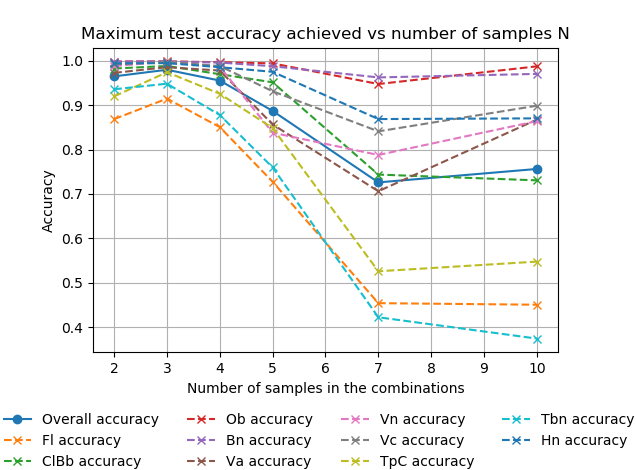
\includegraphics[scale=0.5]{figs/Acc_vs_N_ResNet.png}
\caption{Best overall accuracy and for each instrument obtained by the ResNet depending on the number of instruments in the combinations. \label{best_acc_resnet}}
\end{figure}



\iffalse
\begin{table*}
\center{
\begin{tabular}{|c|c|c|c|c|c|c|c|c|c|c|c|c|c|c|}
\hline
Instruments & \multicolumn{2}{c|}{$N=4$} & \multicolumn{2}{c|}{$N=5$}& \multicolumn{2}{c|}{$N=6$}& \multicolumn{2}{c|}{$N=7$}& \multicolumn{2}{c|}{$N=8$}& \multicolumn{2}{c|}{$N=9$}& \multicolumn{2}{c|}{$N=10$}\\
\cline{2-3} & C & R & C & R & C & R & C & R & C & R & C & R & C & R\\
\hline
All & 0 & 0 & 0 & 0 & 0 & 0 & 0 & 0 & 0 & 0 & 0 & 0 & 0 & 0\\
Hn & 0 & 0 & 0 & 0 & 0 & 0 & 0 & 0 & 0 & 0 & 0 & 0 & 0 & 0\\
Ob & 0 & 0 & 0 & 0 & 0 & 0 & 0 & 0 & 0 & 0 & 0 & 0 & 0 & 0\\
Vn & 0 & 0 & 0 & 0 & 0 & 0 & 0 & 0 & 0 & 0 & 0 & 0 & 0 & 0\\
Va & 0 & 0 & 0 & 0 & 0 & 0 & 0 & 0 & 0 & 0 & 0 & 0 & 0 & 0\\
Vc & 0 & 0 & 0 & 0 & 0 & 0 & 0 & 0 & 0 & 0 & 0 & 0 & 0 & 0\\
Fl & 0 & 0 & 0 & 0 & 0 & 0 & 0 & 0 & 0 & 0 & 0 & 0 & 0 & 0\\
Tbn & 0 & 0 & 0 & 0 & 0 & 0 & 0 & 0 & 0 & 0 & 0 & 0 & 0 & 0\\
Bn & 0 & 0 & 0 & 0 & 0 & 0 & 0 & 0 & 0 & 0 & 0 & 0 & 0 & 0\\
TpC & 0 & 0 & 0 & 0 & 0 & 0 & 0 & 0 & 0 & 0 & 0 & 0 & 0 & 0\\
ClBb & 0 & 0 & 0 & 0 & 0 & 0 & 0 & 0 & 0 & 0 & 0 & 0 & 0 & 0\\
\hline
\end{tabular}

\begin{caption}
Best test accuracy obtained for each model and value of $N$ over the total number of epochs. The accuracy is computed using $f$ define in (\ref{eval}). The first row correspond to the overall accuracy of the model, regrouping all the instruments. C is CNN with LSTM, R is ResNet.
\label{class_res}
\end{caption}}
\end{table*}
\fi

\section{Orchestration experiments}

For orchestrating, we trained our models on combinations of 10 instruments: French Horn, Oboe, Violin, Viola, Cello, Flute, Trombone, Bassoon, Trumpet, and Clarinet. A target sound is input to the model, and the 10 classes with the highest probability are extracted. These 10 classes represent the instrument-note pairs that are most represented in the target, and can be from any combination of the 10 instruments. The dynamic of each sample is inferred from its probability.

We did not train our model to classify the dynamics of a sample despite TinySOL having pianissimo, mezzo forte, and fortissimo recordings for each sample. If we had, then each class would have only one data point: the TinySOL sample ir represents. By not initially ignoring dynamics, this led to each class having three data points: the instrument-note at \textit{pp}, \textit{mf}, and \textit{ff} When the model is used for orchestration, the dynamic is determined by the probability of that sample as output by the model. If the model outputs a probability higher than $0.66$ for a sample, the fortissimo version of the sample was used. If it was between $0.33$ and $0.66$, then the mezzo forte version, and if less than $0.33$ the pianissimo dynamic. The idea behind this is that samples that are the most represented in the target should be the loudest in the orchestrated solution.

We tested our models using 15 targets for orchestration. Two of the targets were made from TinySOL samples, but the rest are not combinations of input data, and some are not even recordings of instruments. Among the targets are recordings of bells, a car horn, a gong, and a recording of a boat docking. 

Although the data we trained the model on was fixed to four seconds of audio, the target samples can be of arbitrary length. By changing the mel hop length, which is the distance between the frames of the melspectrogram, an audio signal of any length can be represented as a matrix of the same size as the training data.

\subsection{Evaluation}

We evaluated our orchestrations both qualitatively and quantitatively. Qualitative evaluation was done through an acoustic inspection of the solution, paying close attention to timbre and pitch. For targets that had harmonic content, it was noted if the partials present in the target were also represented in the orchestrated solution. For example, one of the samples of a bell had partials that represented a C\# minor chord, so we checked if the orchestration contained the notes of the chord. If a target had specific notes, we identified if the note or its partials were present. For example there is target of an Oboe playing an A4 and a Bassoon playing a C\#3, the solution from ResNet contained the partials of the Bassoon's note: C\#3, G\#4, C\#5, and E6 were all included on various instruments in the solution.

For quantitative evaluation, we used the distance metric defined in \eqref{distance} to calculate differences in timbre between targets and solutions. The equation takes in the full FFT of the target and full FFT of the solution. Then for each bin of the FFT, it calculates the absolute difference between the values. The differing values of $\lambda_1$ and $\lambda_2$ allow the metric to penalize the solution in different ways. 

In the summations, all the terms with a $\lambda_1$ will be distances calculated when there was more energy in the target than the solution, since $\delta_{k1} = 1$ only when $x_k \ge \tilde{x}_k$. By the same reasoning, all the terms with a $\lambda_2$ are distances when the solution provided more energy to a frequency than the target; it overshot the frequency. Therefore, the relation between $\lambda_1$ and $\lambda_2$ determines whether a solution is penalized more for undershooting or overshooting the target.

We calculated the distance between the target samples and our orchestrated solutions. We then orchestrated the same targets with OrchIdea and calculated the distance for OrchIdea's solutions. A comparison of these results is in Tab. \ref{orch_eval}.

In order to have comparable solutions, we did not allow OrchIdea to create sparse solutions, meaning that OrchIdea was forced to use all 10 instruments in each solution. This creates a more fair comparison since our model is unable to create sparse solutions.

\begin{equation}\label{distance}
d(x, \tilde{x}) =\lambda_1 \sum_k \delta_{k1}(x_k - \tilde{x}_k) + \lambda_2 \sum_k \delta_{k2}|x_k - \tilde{x	}_k| \\
\end{equation}

\begin{equation}
\delta_{k1} = 
\begin{cases}
1, \text{if   } x_k \ge \tilde{x}_k \\
0, \text{otherwise}
\end{cases} 
\end{equation}

\begin{equation}
\delta_{k2} = 
\begin{cases}
1, \text{if   } x_k < \tilde{x}_k \\
0, \text{otherwise}
\end{cases}
\end{equation}

\begin{table*}
  \begin{center}
    \label{orch_eval}
    \begin{tabular}{|c|c|c|c|c|c|c|c|c|c|} 
    	  \hline
      \textbf{Model} & \textbf{Ob + Bn} & \textbf{Bn} & \textbf{Bass Clarinet} & \textbf{Bell1} & \textbf{Bell2} & \textbf{Yan} & \textbf{Car Horn} & \textbf{Boat} & \textbf{Wind Harp} \\
      \hline
      CNN with LSTM & 0 & 0 & 0 & 0 & 0 & 0 & 0 & 0 & 0\\
      \hline
      ResNet & 0 & 0 & 0 & 0 & 0 & 0 & 0 & 0 & 0 \\
      \hline
      OrchIdea & 0 & 0 & 0 & 0 & 0 & 0 & 0 & 0 & 0  \\
      \hline
    \end{tabular}
  \end{center}
  \caption{Quantitative comparison of orchestrations.}
\end{table*}
\begin{table*}
  \begin{center}
    \label{orch_eval2}
    \begin{tabular}{|c|c|c|c|c|c|c|c|} 
    	  \hline
      \textbf{Model} & \textbf{Chord1} & \textbf{Reed Bone} & \textbf{Chord2} & \textbf{Gong} & \textbf{Scream} & \textbf{Trompe Attack} & \textbf{Average}  \\
      \hline
      CNN with LSTM & 0 & 0 & 0 & 0 & 0 & 0 & 0 \\
      \hline
      ResNet & 0 & 0 & 0 & 0 & 0 & 0 & 0 \\
      \hline
      OrchIdea & 0 & 0 & 0 & 0 & 0 & 0 & 0   \\
      \hline
    \end{tabular}
  \end{center}
  \caption{Continuation of Table 3}
\end{table*}

\section{Conclusion}

Classification through deep learning seems promising for orchestration because of our model's ability to classify individual instruments and pitches out of dense combinations of samples. While our model is not able to outperform OrchIdea, it shows consistent results. When comparing our methods to OrchIdea, it is important to note that many of processes OrchIdea uses to optimize its solution are not present in our model. Our model also lacks the implementation of symbolic constraints, which is an important part of assisted orchestration.\\

We find that the CNN and ResNet give similar accuracies during training, but perform differently when tasked with orchestrating targets. Overall, CNN seems to better emulate the timbre in its orchestrations, where ResNet is better for recreating the harmonic content of the target. 

\subsection{Interpreting the Latent Space}

After training the CNN with LSTM for $N=10$ samples per combination, it is possible to visualize the filters applied to the input layer after layer. Figs. \ref{latent0}-\ref{latent5} show the successive outputs of each layer of the convolutional network. \carmine{I put here all the intermediary features of the CNN with LSTM. I don't find any particular conclusion other than saying that LSTM seems to focus more on vertical components rather than horizontal, ie time over frequency}

\begin{figure}
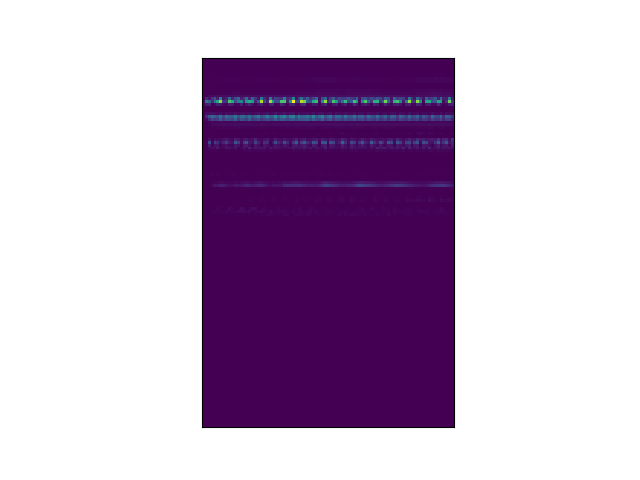
\includegraphics[scale=0.5]{figs/latent_space_layer0.png}
\caption{Initial feature matrix used as input of the model \label{latent0}}
\end{figure}

\begin{figure}
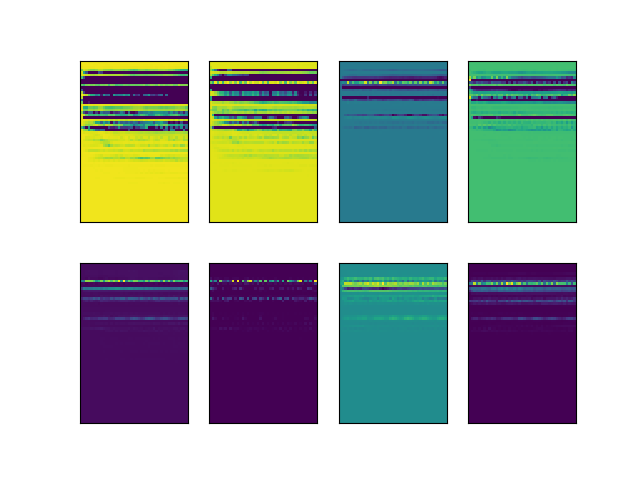
\includegraphics[scale=0.5]{figs/latent_space_layer1.png}
\caption{Intermediary features after the first convolutional layer of the CNN with LSTM. \label{latent1}}
\end{figure}

\begin{figure}
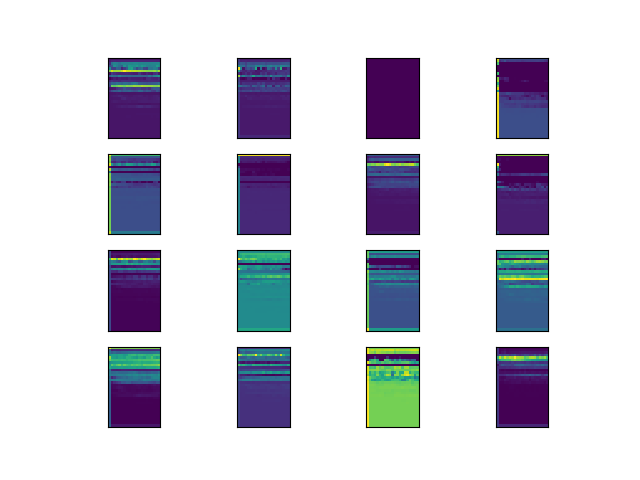
\includegraphics[scale=0.5]{figs/latent_space_layer2.png}
\caption{Intermediary features after the second convolutional layer of the CNN with LSTM. \label{latent2}}
\end{figure}

\begin{figure}
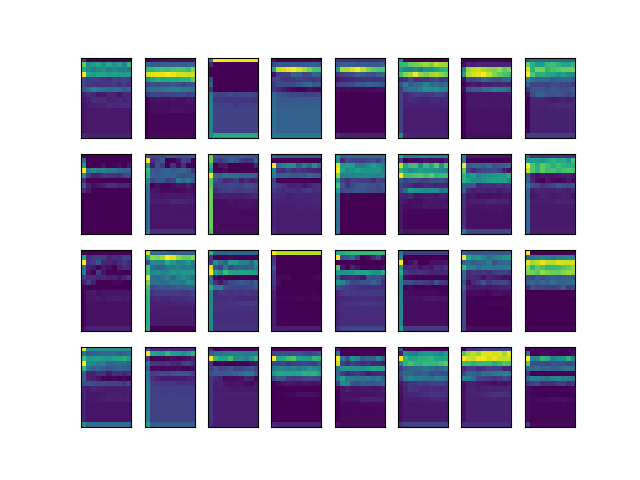
\includegraphics[scale=0.5]{figs/latent_space_layer3.png}
\caption{Intermediary features after the third convolutional layer of the CNN with LSTM. \label{latent3}}
\end{figure}

\begin{figure}
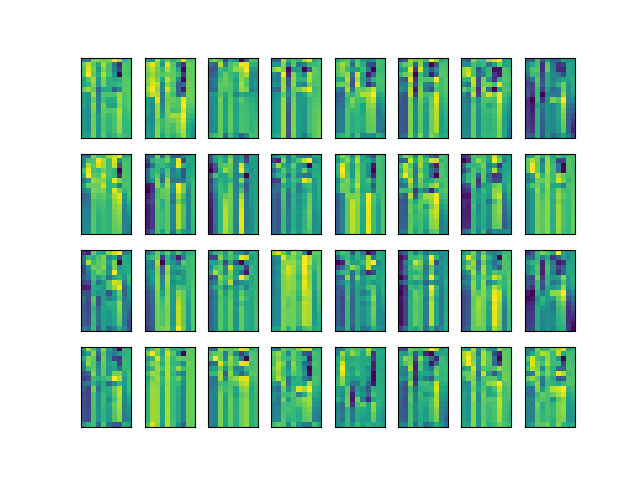
\includegraphics[scale=0.5]{figs/latent_space_layer4.png}
\caption{Intermediary features after the LSTM layer. \label{latent4}}
\end{figure}

\begin{figure}
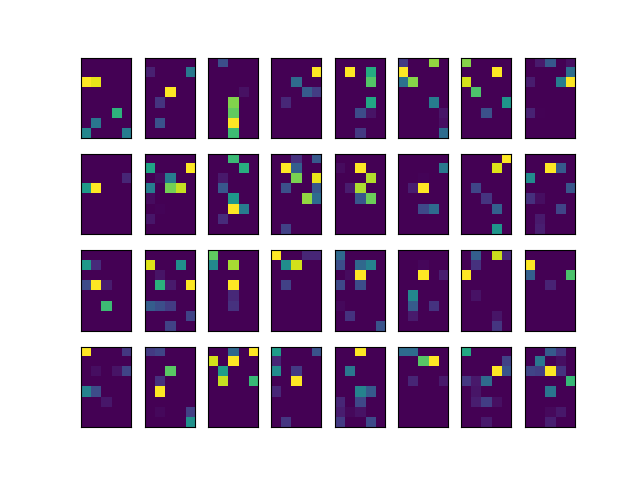
\includegraphics[scale=0.5]{figs/latent_space_layer5.png}
\caption{Intermediary features after final convolutional layer of the CNN with LSTM. \label{latent5}}
\end{figure}

\section{Future steps}

Future steps in this project include implementing various methods that are present in OrchIdea.\\

Our current model orchestrates all targets using the same number of samples, and this does not take into account the density of different targets. The solution to this is to allow sparse solutions in which the model decides how many samples should be used to best represent the target. This allows a small number of samples to be used for sonically sparse sounds and many to be used for sonically dense sounds.\\

Partial filtering is a method that would aid our model in orchestrating the harmonics of a target. The dominant harmonic partials of the target are identified, and the search space is limited to only include samples of those pitches. For example, if the target is a recording of an instrument playing a C4, then the partials identified may be C4, C5, G5, and E6. The model would then only consider samples of these pitches to be used in the solution. This leads to a solution whose harmonics are much closer to the target, which is an important part of aural similarity.

\iffalse
\begin{figure}
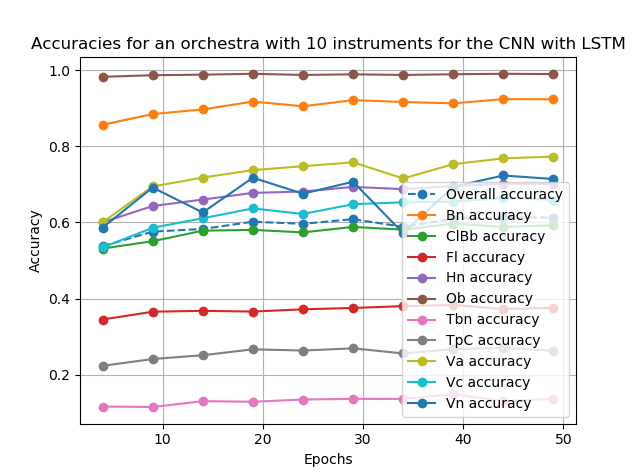
\includegraphics[scale=0.6]{figs/CNN10.png}
\end{figure}
\fi

% For bibtex users:
\bibliography{paper}

% For non bibtex users:
%\begin{thebibliography}{citations}
%
%\bibitem {Author:00}
%E. Author.
%``The Title of the Conference Paper,''
%{\it Proceedings of the International Symposium
%on Music Information Retrieval}, pp.~000--111, 2000.
%
%\bibitem{Someone:10}
%A. Someone, B. Someone, and C. Someone.
%``The Title of the Journal Paper,''
%{\it Journal of New Music Research},
%Vol.~A, No.~B, pp.~111--222, 2010.
%
%\bibitem{Someone:04} X. Someone and Y. Someone. {\it Title of the Book},
%    Editorial Acme, Porto, 2012.
%
%\end{thebibliography}

\end{document}

